\documentclass[usenames, svgnames, dvipsnames]{scrartcl}
\usepackage{pgfplots}
\usepackage{emoji}
\usepackage{siunitx}
\usepackage{ gensymb}
\usepackage[makeroom]{cancel}
% \usepackage{chemformula}
\usepackage[version=3]{mhchem}
\usepackage{simpler-wick}
\newcommand{\ech}{\mathbb{e}}
\newcommand{\gcod}{\mathfrak{D}}
\newcommand{\tz}{{t\tund{0}}}
\newcommand{\php}[1]{\phi_{#1}^+}
\newcommand{\phm}[1]{\phi_{#1}^-}
\newcommand{\fp}{\triangle}
\newcommand{\pho}{\phi_1}
\newcommand{\phii}{\phi_2}
\newcommand{\phiii}{\phi_3}
\newcommand{\phiv}{\phi_4}
\newcommand{\phv}{\phi_5}
\newcommand{\phvi}{\phi_6}
\newcommand{\ti}{{t\tund{1}}}
\newcommand{\tii}{{t\tund{2}}}
\newcommand{\tiii}{{t\tund{3}}}
\newcommand{\tiv}{{t\tund{4}}}
\newcommand{\tv}{{t\tund{5}}}
\usepackage{mathbbol}
\newcommand{\iqe}{iq\ech}
\newcommand{\vph}{\varphi}
\newcommand{\MH}{\mathrm{H}}
\newcommand{\ut}{\uptau}
\newcommand{\phint}{\phi\tund{I}}
\usepackage{simpler-wick}
\usepackage{mathrsfs}
\usepackage{mathtools}
\usepackage{booktabs} % For better table formatting
\usepackage{calc}
\usepackage{Style_File}
\newcommand{\ad}[1]{a_{#1}^\dagger}
\usepackage{fancyhdr}
\newcommand{\pdx}{\vb{p}\cdot \vb{x}}
\newcommand{\creap}{{\hat{a}_{\vb{p}}}^{s\dagger}}
\newcommand{\annap}{{\hat{a}_{\vb{p}}}^{s}}
\newcommand{\crebp}{{\hat{b}_{\vb{p}}}^{s\dagger}}
\newcommand{\annbp}{{\hat{b}_{\vb{p}}}^{s}}


\newcommand{\creapr}{{\hat{a}_{\vb{p}}}^{r\dagger}}
\newcommand{\annapr}{{\hat{a}_{\vb{p}}}^{r}}
\newcommand{\crebpr}{{\hat{b}_{\vb{p}}}^{r\dagger}}
\newcommand{\annbpr}{{\hat{b}_{\vb{p}}}^{r}}
\newcommand{\creampr}{{\hat{a}_{-\vb{p}}}^{r\dagger}}
\newcommand{\annampr}{{\hat{a}_{-\vb{p}}}^{r}}
\newcommand{\crebmpr}{{\hat{b}_{-\vb{p}}}^{r\dagger}}
\newcommand{\annbmpr}{{\hat{b}_{-\vb{p}}}^{r}}
\newcommand{\acomtr}[2]{\{#1,#2\}}
\newcommand{\pdy}{\vb{p}\cdot \vb{y}}
\newcommand{\qdy}{\vb{q}\cdot \vb{y}}

\newcommand{\qdx}{\vb{q}\cdot \vb{x}}
\newcommand{\creaq}{{\hat{a}_{\vb{q}}}^{s\dagger}}
\newcommand{\annaq}{{\hat{a}_{\vb{q}}}^{s}}
\newcommand{\crebq}{{\hat{b}_{\vb{q}}}^{s\dagger}}
\newcommand{\annbq}{{\hat{b}_{\vb{q}}}^{s}}

\newcommand{\creaqr}{{\hat{a}_{\vb{q}}}^{r\dagger}}
\newcommand{\annaqr}{{\hat{a}_{\vb{q}}}^{r}}
\newcommand{\crebqr}{{\hat{b}_{\vb{q}}}^{r\dagger}}
\newcommand{\annbqr}{{\hat{b}_{\vb{q}}}^{r}}

\newcommand{\creamqr}{{\hat{a}_{-\vb{q}}}^{r\dagger}}
\newcommand{\annamqr}{{\hat{a}_{-\vb{q}}}^{r}}
\newcommand{\crebmqr}{{\hat{b}_{-\vb{q}}}^{r\dagger}}
\newcommand{\annbmqr}{{\hat{b}_{-\vb{q}}}^{r}}

% \newcommand{\crebp}{def}
\newenvironment{bMatrix}[1]{%
\bmatrix\array{#1}\hspace*{-0.5\arraycolsep}}%
{\endarray\endbmatrix}
\newcommand{\tund}[1]{_{\text{\tiny #1}}}
\newcommand{\tup}[1]{^{\text{\tiny #1}}}
\newcommand{\uep}{\upepsilon}
\newcommand{\sbo}[1]{\scalebox{0.56}{#1}}
\newcommand{\gsl}[1]{\cancel{#1}}
\usepackage{tensor}
\usepackage{array}
\usepackage{lmodern}
\definecolor{violet}{rgb}{0.5,0.27,0.45}
\newcommand{\hint}{\MH\tund{I}}
\newcommand{\fvec}[1]{\vb{#1}}
\newcommand{\cre}[1]{\hat{a}_{#1}^\dagger}
\newcommand{\ann}[1]{\hat{a}_{#1}}

\newcommand{\crep}{\hat{a}_{\vb{p}}^\dagger}
\newcommand{\annp}{\hat{a}_{\vb{p}}}
\newcommand{\fo}{\hat{\phi}}
\newcommand{\crepd}{\hat{a}_{\vb{p}'}^\dagger}
\newcommand{\annpd}{\hat{a}_{\vb{p}'}}
\newcommand{\vac}{\ket{\Omega}}
\newcommand{\kb}{k\tund{B}}
\newcommand{\vacb}{\bra{\Omega}}
\newcommand{\cremp}{\hat{a}_{\vb{-p}}^\dagger}
\newcommand{\annmp}{\hat{a}_{\vb{-p}}}

\newcommand{\crempd}{\hat{a}_{\vb{-p}'}^\dagger}
\newcommand{\annmpd}{\hat{a}_{\vb{-p}'}}

\newcommand{\tvec}[1]{\vb{{#1}}}
\renewcommand{\aa}[1]{a_{#1}}
\newcommand{\overbar}[1]{\mkern 1.5mu\overline{\mkern-1.5mu{#1}\mkern-1.5mu}\mkern 1.5mu}
\newcommand{\dadj}[1]{\overbar{#1}}
\newcommand{\bili}[1]{\dadj{\Psi}\ #1 \ \Psi}
\newcommand{\bilin}[3]{\dadj{\Psi}_{#1}\ #3 \ \Psi_{#2}}
\newcommand{\lrep}{\mathrm{S}[\Lambda]}
\newcommand{\lrepd}{\mathrm{S}^\dagger[\Lambda]}
\newcommand{\lrepinv}{\mathrm{S}^{-1}[\Lambda]}
\newcolumntype{P}[1]{>{\centering\arraybackslash}p{#1}}
% Recommended preamble:
\usetikzlibrary{arrows.meta}
\usetikzlibrary{backgrounds}
\usepgfplotslibrary{patchplots}
\usepgfplotslibrary{fillbetween}
\pgfplotsset{%
    layers/standard/.define layer set={%
        background,axis background,axis grid,axis ticks,axis lines,axis tick labels,pre main,main,axis descriptions,axis foreground%
    }{
        grid style={/pgfplots/on layer=axis grid},%
        tick style={/pgfplots/on layer=axis ticks},%
        axis line style={/pgfplots/on layer=axis lines},%
        label style={/pgfplots/on layer=axis descriptions},%
        legend style={/pgfplots/on layer=axis descriptions},%
        title style={/pgfplots/on layer=axis descriptions},%
        colorbar style={/pgfplots/on layer=axis descriptions},%
        ticklabel style={/pgfplots/on layer=axis tick labels},%
        axis background@ style={/pgfplots/on layer=axis background},%
        3d box foreground style={/pgfplots/on layer=axis foreground},%
    },
}
\newcommand{\amstitle}[1]{%
  {\Large\MakeUppercase{#1}}% First letter large, rest small caps (simplified)
  % OR for true small caps:
  % {\Large\MakeUppercase{\expandafter\@firstofone#1}\scshape\MakeLowercase{#1}}%
}
\usepackage[left = 0.8in,
right = 0.6in,
bottom = 0.8in,
top = 0.8in,
a4paper]{geometry}

\lstdefinelanguage{Julia}{
  morekeywords={
    abstract, break, case, catch, const, continue, do, else, elseif,
    end, export, false, for, function, global, if, import, in, let,
    local, macro, module, mutable, new, quote, return, true, try,
    type, using, while, where, struct
  },
  sensitive=true,
  morecomment=[l]\#,
  morestring=[b]",
}
\usepackage{listings}
\lstset{
  language=Julia,
  basicstyle=\ttfamily\footnotesize,
  keywordstyle=\color{blue}\bfseries,
  commentstyle=\color{gray},
  stringstyle=\color{red},
  breaklines=true,
  breakatwhitespace=true,
  showstringspaces=false,
  frame=single,
  columns=fullflexible,
  captionpos=b
}

\fancyhead[L,C]{}
\fancyhead[R]{Lab Report}
\usepackage[hidelinks]{hyperref}
\hypersetup{colorlinks=true,linkcolor=cyan!80!black, citecolor=YellowOrange,urlcolor=cyan!80!black}
\usepackage{doi}
\fancyhead[L]{ PH4201}
\fancyhead[C]{Adv. Optics Lab}
\fancyfoot[C]{\thepage}
\fancyfoot[R,L]{}
\usetikzlibrary{calc}
\pagestyle{fancy}
\newcommand{\delt}[2]{\tensor{\delta}{^{#1}_{#2}}}
\newcommand{\vact}{\ket{\widetilde{\Omega}}}
\newcommand{\vactb}{\bra{\widetilde{\Omega}}}
\newcommand{\meas}[1]{\frac{\dd^3\tvec{#1}}{(2\pi)^3}}
\newcommand{\tvp}{\tvec{p}}
\newcommand{\tvpd}{\tvec{p}'}
\newcommand{\ddelt}[1]{\delta^{(3)}(#1)}
\newcommand{\myeq}[1]{\stackrel{\mathclap{\tiny\mbox{#1}}}{=}}
\newcommand{\omp}{\omega_{\tvp}}
\newcommand{\ompd}{\omega_{\tvpd}}
\renewcommand{\headrulewidth}{0.4pt}
\definecolor{titleblue}{RGB}{0, 80, 120}
\usepackage{longtable} 

\renewcommand{\fdv}[2]{\frac{\delta #1}{\delta #2}}
\begin{document}
        \begin{center}
            {\rmfamily
                \Large{\textcolor{blue!30!black}{%
                    \textmd{{\Large{{S}}}}patial \textmd{{\Large{{L}}}}ight \textmd{{\Large{{M}}}}odulation \\
                     {\Large Experiment} 04%
                }}\\[0.4cm]
            }
            \end{center}
        \begin{center}
           \large \texttt{{{\LARGE  S}agnik {\LARGE S}eth\hspace{0.3cm} 22MS026 \hspace{0.3cm} Group:B6}}
        \end{center}
\hrule
\vspace{0.08cm}
\hrule
\vspace{0.6cm}
\section{Aim}
 To measure the linear retardance and optical rotation of a SLM device for various grey scale values.

\section{Apparatus}
The required apparatus for performing the experiment are:
\begin{multicols}{3}
\begin{enumerate}
  \item Laser source
  \item SLM device 
  \item Polarizers 
  \item Glass Slab
  \item Neutral-density filter
  \item Current detector
\end{enumerate}
\end{multicols}

\section{Theory}
\subsection{Polarization of Light}
Light is a transverse electromagnetic wave. For a wave travelling in in the $\hat{z}$ direction we have,
\begin{equation}
E_x = E_{0x} e^{i(\omega t - kz + \delta_x)}, \quad
E_y = E_{0y} e^{i(\omega t - kz + \delta_y)}
\end{equation}
Depending on the amplitudes and phase difference between the components of the electric field, we define different polarizations viz. linear, circular, or elliptical.

\subsection{Stokes Parameters and Mueller Matrices}
The complete description of the polarization state is given by the Stokes vector, based on the intensity parameters:
\begin{equation}\label{stokes}
S =
\begin{bmatrix}
S\tund{0} \\
S\tund{1} \\
S\tund{2} \\
S\tund{3}
\end{bmatrix}
=
\begin{bmatrix}
I_H + I_V \\
I_H - I_V \\
I_P - I_M \\
I_R - I_L
\end{bmatrix}
\end{equation}
where $S\tund{0}$ is the total intensity of the beam,  $S\tund{1}$ represents the difference of intensities in the horizontal or vertical polarization ($I_H - I_V$), $S\tund{2}$ denotes the difference in intensities between  $+45\degree$ or $-45\degree$ polarization states (($I_P - I_M$)) while $S\tund{3}$ represents the difference in intensities of the circular polarization states ($I_R - I_L$).
\noindent
The interaction of polarized light with an optical element can be described by the Mueller matrix $M$:
\begin{equation}
S_{\text{out}} = \mathrm{M} S_{\text{in}}\qquad M \equiv
\begin{bmatrix}
m_{11} & m_{12} & m_{13} & m_{14} \\
m_{21} & m_{22} & m_{23} & m_{24} \\
m_{31} & m_{32} & m_{33} & m_{34} \\
m_{41} & m_{42} & m_{43} & m_{44}
\end{bmatrix}
\end{equation}
where $S_{\text{in}}$ and $S_{\text{out}}$ are the input and output Stokes vectors.
\subsubsection{Mueller Matrix of a Linear Retarder}
An important property of an optical medium is \textit{retardance}, which arises due to the difference in the refractive index of two orthogonal polarization states and results in a phase difference. For a linear retarder with retardance $\delta$ and fast axis at angle $\theta$:

\begin{equation}
M_{\text{lin}} =
\begin{bmatrix}
1 & 0 & 0 & 0 \\
0 & \cos^2 2\theta + \cos\delta \sin^2 2\theta & (1-\cos\delta)\sin 2\theta \cos 2\theta & -\sin\delta \sin 2\theta \\
0 & (1-\cos\delta)\sin 2\theta \cos 2\theta & \sin^2 2\theta + \cos\delta \cos^2 2\theta & \sin\delta \cos 2\theta \\
0 & \sin\delta \sin 2\theta & -\sin\delta \cos 2\theta & \cos\delta
\end{bmatrix}
\end{equation}

\subsubsection{Mueller Matrix of a Circular Retarder (Optical Rotator)}
For optical rotation by an angle $\psi$, the Mueller matrix becomes:
\begin{equation}
M_{\text{circ}} =
\begin{bmatrix}
1 & 0 & 0 & 0 \\
0 & \cos 2\psi & \sin 2\psi & 0 \\
0 & -\sin 2\psi & \cos 2\psi & 0 \\
0 & 0 & 0 & 1
\end{bmatrix}
\end{equation}

\subsubsection{Mueller Matrix of SLM}
Spatial Light Modulator is a optoelectronic device, containing twisted layers of liquid crystals and is used to modulate the magnitude or phase of a beam of light. Electric field can be applied to tilt these crystals to produce the intended effect. SLM behaves as a combination of a linear retarder and an optical rotator:
\begin{equation}
M_{\text{SLM}} = M_{\text{circ}} \cdot M_{\text{lin}}
\end{equation}
Thus, the SLM introduces both retardance ($\delta$) and optical rotation ($\psi$), which are determined experimentally using Stokes measurements. For horizontal incident light, the output Stokes vector is, 
\begin{equation}
    S\tund{1} = \mqty[1 \\ \cos 2\theta \cos(2\theta-2\psi)+\sin 2\theta\cos\delta \sin(2\theta-2\psi)\\ \sin 2\theta \cos(2\theta-2\psi)-\cos 2\theta\cos\delta \sin(2\theta-2\psi)\\ \sin(2\theta-2\psi)]
\end{equation}
For the $+45\degree$ polarization, the output Stokes vector is given by, 
\begin{equation}
    S\tund{2} = \mqty[1 \\ \cos 2\theta \sin(2\theta-2\psi)-\sin 2\theta\cos\delta \cos(2\theta-2\psi)\\ \sin 2\theta \sin(2\theta-2\psi)+\cos 2\theta\cos\delta \cos(2\theta-2\psi)\\ -\cos(2\theta-2\psi)\sin \delta]
\end{equation}
From this we calculate the linear retardance $\delta$ and the rotation $\psi$ of an SLM by,
\begin{align}
   \begin{split}
     [S\tund{1}]_2+[S\tund{2}]_3 = (1+\cos \delta)\cos 2\psi=X\\
     [S\tund{1}]_3-[S\tund{2}]_2= (1+\cos \delta)\sin 2\psi=Y
   \end{split}
\end{align}
where $[S\tund{i}]_j $ is the $j^{\text{th}}$ component of $S\tund{i}$ vector. Simplifying this gives us, 
\begin{align}
    \delta = \cos^{-1}\qty[\sqrt{X^2+Y^2}-1] \qquad \psi = \tan^{-1}\qty(\frac{Y}{X})
\end{align}
\section{Brewster's Angle}
To determine the polarization axis of the given polarizer, we need to use the concept of Brewster's angle, which is the angle of incidence at which light of a particular polarization will transmit fully through a dielectric surface. If unpolarized light is incident, it becomes polarized after reflection from the surface.
\begin{figure}[H]
    \centering
    

% Gradient Info
  
\tikzset {_7nwa4bp0l/.code = {\pgfsetadditionalshadetransform{ \pgftransformshift{\pgfpoint{0 bp } { 0 bp }  }  \pgftransformrotate{0 }  \pgftransformscale{2 }  }}}
\pgfdeclarehorizontalshading{_pq4neehle}{150bp}{rgb(0bp)=(0.94,0.98,1);
rgb(37.5bp)=(0.94,0.98,1);
rgb(49.25bp)=(0.8,0.92,1);
rgb(62.5bp)=(0.63,0.86,1);
rgb(100bp)=(0.63,0.86,1)}

% Pattern Info
 
\tikzset{
pattern size/.store in=\mcSize, 
pattern size = 5pt,
pattern thickness/.store in=\mcThickness, 
pattern thickness = 0.3pt,
pattern radius/.store in=\mcRadius, 
pattern radius = 1pt}
\makeatletter
\pgfutil@ifundefined{pgf@pattern@name@_vvonuzueu}{
\pgfdeclarepatternformonly[\mcThickness,\mcSize]{_vvonuzueu}
{\pgfqpoint{0pt}{0pt}}
{\pgfpoint{\mcSize+\mcThickness}{\mcSize+\mcThickness}}
{\pgfpoint{\mcSize}{\mcSize}}
{
\pgfsetcolor{\tikz@pattern@color}
\pgfsetlinewidth{\mcThickness}
\pgfpathmoveto{\pgfqpoint{0pt}{0pt}}
\pgfpathlineto{\pgfpoint{\mcSize+\mcThickness}{\mcSize+\mcThickness}}
\pgfusepath{stroke}
}}
\makeatother
\tikzset{every picture/.style={line width=0.75pt}} %set default line width to 0.75pt        

\begin{tikzpicture}[x=0.75pt,y=0.75pt,yscale=-1,xscale=1]
%uncomment if require: \path (0,300); %set diagram left start at 0, and has height of 300

%Shape: Rectangle [id:dp413017015080824] 
\path  [shading=_pq4neehle,_7nwa4bp0l] (102.68,109.39) -- (341.87,109.39) -- (341.87,168.51) -- (102.68,168.51) -- cycle ; % for fading 
 \draw   (102.68,109.39) -- (341.87,109.39) -- (341.87,168.51) -- (102.68,168.51) -- cycle ; % for border 

%Straight Lines [id:da18616624655167613] 
\draw    (89.4,39.13) -- (218.29,109.39) ;
%Straight Lines [id:da21854156531225666] 
\draw    (219.62,109.39) -- (328.17,48.55) ;
\draw [shift={(329.91,47.57)}, rotate = 150.73] [color={rgb, 255:red, 0; green, 0; blue, 0 }  ][line width=0.75]    (6.56,-1.97) .. controls (4.17,-0.84) and (1.99,-0.18) .. (0,0) .. controls (1.99,0.18) and (4.17,0.84) .. (6.56,1.97)   ;
%Straight Lines [id:da6409282231378658] 
\draw    (219.62,109.39) -- (264.8,162.95) ;
%Straight Lines [id:da6348939292931102] 
\draw  [dash pattern={on 4.5pt off 4.5pt}]  (218.29,39.45) -- (219.62,186.78) ;
%Straight Lines [id:da056960559798641786] 
\draw    (123.68,43.78) -- (108.88,62.5) ;
\draw [shift={(107.64,64.07)}, rotate = 308.31] [color={rgb, 255:red, 0; green, 0; blue, 0 }  ][line width=0.75]    (4.37,-1.32) .. controls (2.78,-0.56) and (1.32,-0.12) .. (0,0) .. controls (1.32,0.12) and (2.78,0.56) .. (4.37,1.32)   ;
\draw [shift={(124.92,42.21)}, rotate = 128.31] [color={rgb, 255:red, 0; green, 0; blue, 0 }  ][line width=0.75]    (4.37,-1.32) .. controls (2.78,-0.56) and (1.32,-0.12) .. (0,0) .. controls (1.32,0.12) and (2.78,0.56) .. (4.37,1.32)   ;
%Straight Lines [id:da4784529997211655] 
\draw    (139.98,53.74) -- (125.18,72.47) ;
\draw [shift={(123.94,74.04)}, rotate = 308.31] [color={rgb, 255:red, 0; green, 0; blue, 0 }  ][line width=0.75]    (4.37,-1.32) .. controls (2.78,-0.56) and (1.32,-0.12) .. (0,0) .. controls (1.32,0.12) and (2.78,0.56) .. (4.37,1.32)   ;
\draw [shift={(141.22,52.17)}, rotate = 128.31] [color={rgb, 255:red, 0; green, 0; blue, 0 }  ][line width=0.75]    (4.37,-1.32) .. controls (2.78,-0.56) and (1.32,-0.12) .. (0,0) .. controls (1.32,0.12) and (2.78,0.56) .. (4.37,1.32)   ;
%Straight Lines [id:da3390173320696227] 
\draw    (157.25,62.81) -- (142.46,81.53) ;
\draw [shift={(141.22,83.1)}, rotate = 308.31] [color={rgb, 255:red, 0; green, 0; blue, 0 }  ][line width=0.75]    (4.37,-1.32) .. controls (2.78,-0.56) and (1.32,-0.12) .. (0,0) .. controls (1.32,0.12) and (2.78,0.56) .. (4.37,1.32)   ;
\draw [shift={(158.49,61.24)}, rotate = 128.31] [color={rgb, 255:red, 0; green, 0; blue, 0 }  ][line width=0.75]    (4.37,-1.32) .. controls (2.78,-0.56) and (1.32,-0.12) .. (0,0) .. controls (1.32,0.12) and (2.78,0.56) .. (4.37,1.32)   ;
%Straight Lines [id:da7981775843954084] 
\draw    (175.86,73.04) -- (161.06,91.76) ;
\draw [shift={(159.82,93.33)}, rotate = 308.31] [color={rgb, 255:red, 0; green, 0; blue, 0 }  ][line width=0.75]    (4.37,-1.32) .. controls (2.78,-0.56) and (1.32,-0.12) .. (0,0) .. controls (1.32,0.12) and (2.78,0.56) .. (4.37,1.32)   ;
\draw [shift={(177.1,71.47)}, rotate = 128.31] [color={rgb, 255:red, 0; green, 0; blue, 0 }  ][line width=0.75]    (4.37,-1.32) .. controls (2.78,-0.56) and (1.32,-0.12) .. (0,0) .. controls (1.32,0.12) and (2.78,0.56) .. (4.37,1.32)   ;
%Straight Lines [id:da24171535124748034] 
\draw    (193.13,82.04) -- (178.34,100.77) ;
\draw [shift={(177.1,102.34)}, rotate = 308.31] [color={rgb, 255:red, 0; green, 0; blue, 0 }  ][line width=0.75]    (4.37,-1.32) .. controls (2.78,-0.56) and (1.32,-0.12) .. (0,0) .. controls (1.32,0.12) and (2.78,0.56) .. (4.37,1.32)   ;
\draw [shift={(194.37,80.47)}, rotate = 128.31] [color={rgb, 255:red, 0; green, 0; blue, 0 }  ][line width=0.75]    (4.37,-1.32) .. controls (2.78,-0.56) and (1.32,-0.12) .. (0,0) .. controls (1.32,0.12) and (2.78,0.56) .. (4.37,1.32)   ;
%Straight Lines [id:da8427357694311791] 
\draw    (248.91,121.25) -- (226.08,131.7) ;
\draw [shift={(224.26,132.53)}, rotate = 335.41] [color={rgb, 255:red, 0; green, 0; blue, 0 }  ][line width=0.75]    (4.37,-1.32) .. controls (2.78,-0.56) and (1.32,-0.12) .. (0,0) .. controls (1.32,0.12) and (2.78,0.56) .. (4.37,1.32)   ;
\draw [shift={(250.73,120.42)}, rotate = 155.41] [color={rgb, 255:red, 0; green, 0; blue, 0 }  ][line width=0.75]    (4.37,-1.32) .. controls (2.78,-0.56) and (1.32,-0.12) .. (0,0) .. controls (1.32,0.12) and (2.78,0.56) .. (4.37,1.32)   ;
%Straight Lines [id:da9176594133907106] 
\draw    (259.3,137.06) -- (236.46,147.51) ;
\draw [shift={(234.64,148.34)}, rotate = 335.41] [color={rgb, 255:red, 0; green, 0; blue, 0 }  ][line width=0.75]    (4.37,-1.32) .. controls (2.78,-0.56) and (1.32,-0.12) .. (0,0) .. controls (1.32,0.12) and (2.78,0.56) .. (4.37,1.32)   ;
\draw [shift={(261.12,136.23)}, rotate = 155.41] [color={rgb, 255:red, 0; green, 0; blue, 0 }  ][line width=0.75]    (4.37,-1.32) .. controls (2.78,-0.56) and (1.32,-0.12) .. (0,0) .. controls (1.32,0.12) and (2.78,0.56) .. (4.37,1.32)   ;
%Straight Lines [id:da0947961125232677] 
\draw    (269.98,152.35) -- (247.14,162.8) ;
\draw [shift={(245.33,163.64)}, rotate = 335.41] [color={rgb, 255:red, 0; green, 0; blue, 0 }  ][line width=0.75]    (4.37,-1.32) .. controls (2.78,-0.56) and (1.32,-0.12) .. (0,0) .. controls (1.32,0.12) and (2.78,0.56) .. (4.37,1.32)   ;
\draw [shift={(271.8,151.52)}, rotate = 155.41] [color={rgb, 255:red, 0; green, 0; blue, 0 }  ][line width=0.75]    (4.37,-1.32) .. controls (2.78,-0.56) and (1.32,-0.12) .. (0,0) .. controls (1.32,0.12) and (2.78,0.56) .. (4.37,1.32)   ;
%Shape: Ellipse [id:dp28722941764418075] 
\draw  [fill={rgb, 255:red, 0; green, 0; blue, 0 }  ,fill opacity=1 ] (237.08,98.72) .. controls (237.08,97.56) and (238.11,96.63) .. (239.38,96.63) .. controls (240.66,96.63) and (241.69,97.56) .. (241.69,98.72) .. controls (241.69,99.87) and (240.66,100.81) .. (239.38,100.81) .. controls (238.11,100.81) and (237.08,99.87) .. (237.08,98.72) -- cycle ;
%Shape: Ellipse [id:dp3736061102557904] 
\draw  [fill={rgb, 255:red, 0; green, 0; blue, 0 }  ,fill opacity=1 ] (113.98,53.14) .. controls (113.98,51.99) and (115.01,51.05) .. (116.28,51.05) .. controls (117.55,51.05) and (118.59,51.99) .. (118.59,53.14) .. controls (118.59,54.29) and (117.55,55.23) .. (116.28,55.23) .. controls (115.01,55.23) and (113.98,54.29) .. (113.98,53.14) -- cycle ;
%Shape: Ellipse [id:dp4185458018636755] 
\draw  [fill={rgb, 255:red, 0; green, 0; blue, 0 }  ,fill opacity=1 ] (130.28,63.11) .. controls (130.28,61.95) and (131.31,61.02) .. (132.58,61.02) .. controls (133.85,61.02) and (134.89,61.95) .. (134.89,63.11) .. controls (134.89,64.26) and (133.85,65.2) .. (132.58,65.2) .. controls (131.31,65.2) and (130.28,64.26) .. (130.28,63.11) -- cycle ;
%Shape: Ellipse [id:dp7631425604438481] 
\draw  [fill={rgb, 255:red, 0; green, 0; blue, 0 }  ,fill opacity=1 ] (147.55,72.17) .. controls (147.55,71.02) and (148.58,70.08) .. (149.86,70.08) .. controls (151.13,70.08) and (152.16,71.02) .. (152.16,72.17) .. controls (152.16,73.33) and (151.13,74.26) .. (149.86,74.26) .. controls (148.58,74.26) and (147.55,73.33) .. (147.55,72.17) -- cycle ;
%Shape: Ellipse [id:dp38816884133619145] 
\draw  [fill={rgb, 255:red, 0; green, 0; blue, 0 }  ,fill opacity=1 ] (166.16,82.4) .. controls (166.16,81.25) and (167.19,80.31) .. (168.46,80.31) .. controls (169.73,80.31) and (170.76,81.25) .. (170.76,82.4) .. controls (170.76,83.55) and (169.73,84.49) .. (168.46,84.49) .. controls (167.19,84.49) and (166.16,83.55) .. (166.16,82.4) -- cycle ;
%Shape: Ellipse [id:dp38457739504592114] 
\draw  [fill={rgb, 255:red, 0; green, 0; blue, 0 }  ,fill opacity=1 ] (183.43,91.4) .. controls (183.43,90.25) and (184.46,89.31) .. (185.74,89.31) .. controls (187.01,89.31) and (188.04,90.25) .. (188.04,91.4) .. controls (188.04,92.56) and (187.01,93.49) .. (185.74,93.49) .. controls (184.46,93.49) and (183.43,92.56) .. (183.43,91.4) -- cycle ;
%Shape: Ellipse [id:dp437087697434131] 
\draw  [fill={rgb, 255:red, 0; green, 0; blue, 0 }  ,fill opacity=1 ] (255.68,87.86) .. controls (255.68,86.71) and (256.71,85.77) .. (257.99,85.77) .. controls (259.26,85.77) and (260.29,86.71) .. (260.29,87.86) .. controls (260.29,89.02) and (259.26,89.95) .. (257.99,89.95) .. controls (256.71,89.95) and (255.68,89.02) .. (255.68,87.86) -- cycle ;
%Shape: Ellipse [id:dp7388494608806288] 
\draw  [fill={rgb, 255:red, 0; green, 0; blue, 0 }  ,fill opacity=1 ] (272.46,78.48) .. controls (272.46,77.33) and (273.5,76.39) .. (274.77,76.39) .. controls (276.04,76.39) and (277.07,77.33) .. (277.07,78.48) .. controls (277.07,79.64) and (276.04,80.57) .. (274.77,80.57) .. controls (273.5,80.57) and (272.46,79.64) .. (272.46,78.48) -- cycle ;
%Shape: Ellipse [id:dp9712376588270861] 
\draw  [fill={rgb, 255:red, 0; green, 0; blue, 0 }  ,fill opacity=1 ] (288.41,69.72) .. controls (288.41,68.56) and (289.44,67.63) .. (290.71,67.63) .. controls (291.99,67.63) and (293.02,68.56) .. (293.02,69.72) .. controls (293.02,70.87) and (291.99,71.81) .. (290.71,71.81) .. controls (289.44,71.81) and (288.41,70.87) .. (288.41,69.72) -- cycle ;
%Shape: Ellipse [id:dp47824482934757206] 
\draw  [fill={rgb, 255:red, 0; green, 0; blue, 0 }  ,fill opacity=1 ] (305.69,60.07) .. controls (305.69,58.92) and (306.72,57.98) .. (307.99,57.98) .. controls (309.26,57.98) and (310.29,58.92) .. (310.29,60.07) .. controls (310.29,61.23) and (309.26,62.16) .. (307.99,62.16) .. controls (306.72,62.16) and (305.69,61.23) .. (305.69,60.07) -- cycle ;
%Shape: Ellipse [id:dp4919170154902677] 
\draw  [fill={rgb, 255:red, 0; green, 0; blue, 0 }  ,fill opacity=1 ] (251.2,149.3) .. controls (251.2,148.15) and (252.23,147.21) .. (253.51,147.21) .. controls (254.78,147.21) and (255.81,148.15) .. (255.81,149.3) .. controls (255.81,150.45) and (254.78,151.39) .. (253.51,151.39) .. controls (252.23,151.39) and (251.2,150.45) .. (251.2,149.3) -- cycle ;
\draw   (102.45,40.05) -- (103.11,46.93) -- (95.51,47.35) ;
%Shape: Arc [id:dp3177344413986858] 
\draw  [draw opacity=0] (206.61,101.75) .. controls (209.28,98.01) and (213.86,95.49) .. (219.09,95.33) -- (219.62,109.39) -- cycle ; \draw   (206.61,101.75) .. controls (209.28,98.01) and (213.86,95.49) .. (219.09,95.33) ;  
%Shape: Rectangle [id:dp19044532861121366] 
\draw  [pattern=_vvonuzueu,pattern size=6pt,pattern thickness=0.75pt,pattern radius=0pt, pattern color={rgb, 255:red, 0; green, 0; blue, 0}] (371.18,68.55) -- (364.14,74.06) -- (312.8,20) -- (319.85,14.49) -- cycle ;

% Text Node
\draw (203.32,83.69) node [anchor=north west][inner sep=0.75pt]  [font=\scriptsize]  {$\theta $};
% Text Node
\draw (109.78,91.03) node [anchor=north west][inner sep=0.75pt]  [font=\scriptsize]  {$n_{1}$};
% Text Node
\draw (112.43,141.67) node [anchor=north west][inner sep=0.75pt]  [font=\scriptsize]  {$n_{2}$};
% Text Node
\draw (144.65,28.79) node [anchor=north west][inner sep=0.75pt]  [font=\scriptsize,rotate=-31.68] [align=left] {(unpolarised)};
% Text Node
\draw (242.32,61.53) node [anchor=north west][inner sep=0.75pt]  [font=\scriptsize,rotate=-328.32] [align=left] {(polarised)};
% Text Node
\draw (350.83,17.42) node [anchor=north west][inner sep=0.75pt]  [font=\scriptsize,rotate=-49.25] [align=left] {Detector};
% Text Node
\draw (279.63,177.34) node [anchor=north west][inner sep=0.75pt]  [font=\scriptsize] [align=left] {Glass Slab};


\end{tikzpicture}

\end{figure}
\noindent
If light is going from a medium with refective index $n\tund{1}$ to a medium of refractive index $n\tund{2}$ then Brewster's angle is given by, 
\begin{equation}
    \theta\tund{B} = \tan^{-1}\qty(\frac{n\tund{1}}{n\tund{2}})
\end{equation}
The experiment consists of two parts, first we determine the polarisation axis of the two polarizers using Brewster's angle.
\begin{figure}[H]
    \centering 
    

% Gradient Info
  
\tikzset {_bfsmqoecl/.code = {\pgfsetadditionalshadetransform{ \pgftransformshift{\pgfpoint{0 bp } { 0 bp }  }  \pgftransformrotate{0 }  \pgftransformscale{2 }  }}}
\pgfdeclarehorizontalshading{_edhldii6a}{150bp}{rgb(0bp)=(0.88,1,1);
rgb(37.5bp)=(0.88,1,1);
rgb(39.25bp)=(0.88,1,1);
rgb(40.5bp)=(0.99,1,1);
rgb(45bp)=(0.9,0.97,0.99);
rgb(51bp)=(0.78,0.93,0.98);
rgb(56.25bp)=(0.75,0.89,0.97);
rgb(62.5bp)=(0.69,0.85,0.96);
rgb(100bp)=(0.69,0.85,0.96)}

% Pattern Info
 
\tikzset{
pattern size/.store in=\mcSize, 
pattern size = 5pt,
pattern thickness/.store in=\mcThickness, 
pattern thickness = 0.3pt,
pattern radius/.store in=\mcRadius, 
pattern radius = 1pt}
\makeatletter
\pgfutil@ifundefined{pgf@pattern@name@_zk9c4qp4q}{
\pgfdeclarepatternformonly[\mcThickness,\mcSize]{_zk9c4qp4q}
{\pgfqpoint{0pt}{0pt}}
{\pgfpoint{\mcSize+\mcThickness}{\mcSize+\mcThickness}}
{\pgfpoint{\mcSize}{\mcSize}}
{
\pgfsetcolor{\tikz@pattern@color}
\pgfsetlinewidth{\mcThickness}
\pgfpathmoveto{\pgfqpoint{0pt}{0pt}}
\pgfpathlineto{\pgfpoint{\mcSize+\mcThickness}{\mcSize+\mcThickness}}
\pgfusepath{stroke}
}}
\makeatother
\tikzset{every picture/.style={line width=0.75pt}} %set default line width to 0.75pt        

\begin{tikzpicture}[x=0.75pt,y=0.75pt,yscale=-1,xscale=1]
%uncomment if require: \path (0,214); %set diagram left start at 0, and has height of 214

%Shape: Square [id:dp3600650713538579] 
\draw  [fill={rgb, 255:red, 192; green, 247; blue, 136 }  ,fill opacity=1 ] (104,138) -- (128,138) -- (128,162) -- (104,162) -- cycle ;
%Flowchart: Terminator [id:dp7824235036188806] 
\path  [shading=_edhldii6a,_bfsmqoecl] (248,170.75) -- (248,131.43) .. controls (248,126.32) and (250.91,122.18) .. (254.5,122.18) .. controls (258.09,122.18) and (261,126.32) .. (261,131.43) -- (261,170.75) .. controls (261,175.86) and (258.09,180) .. (254.5,180) .. controls (250.91,180) and (248,175.86) .. (248,170.75) -- cycle ; % for fading 
 \draw   (248,170.75) -- (248,131.43) .. controls (248,126.32) and (250.91,122.18) .. (254.5,122.18) .. controls (258.09,122.18) and (261,126.32) .. (261,131.43) -- (261,170.75) .. controls (261,175.86) and (258.09,180) .. (254.5,180) .. controls (250.91,180) and (248,175.86) .. (248,170.75) -- cycle ; % for border 

%Shape: Ellipse [id:dp005570376497502472] 
\draw  [fill={rgb, 255:red, 247; green, 237; blue, 157 }  ,fill opacity=1 ] (335,173) .. controls (329.48,173) and (325,163.07) .. (325,150.82) .. controls (325,138.57) and (329.48,128.63) .. (335,128.63) .. controls (340.52,128.63) and (345,138.57) .. (345,150.82) .. controls (345,163.07) and (340.52,173) .. (335,173) -- cycle ;
%Shape: Ellipse [id:dp055503989269594545] 
\draw  [fill={rgb, 255:red, 247; green, 237; blue, 157 }  ,fill opacity=1 ] (174,174) .. controls (168.48,174) and (164,164.07) .. (164,151.82) .. controls (164,139.57) and (168.48,129.63) .. (174,129.63) .. controls (179.52,129.63) and (184,139.57) .. (184,151.82) .. controls (184,164.07) and (179.52,174) .. (174,174) -- cycle ;
%Straight Lines [id:da9916632038936388] 
\draw  [dash pattern={on 4.5pt off 4.5pt}]  (84,150.25) -- (380,150.18) ;
\draw [shift={(382,150.18)}, rotate = 179.99] [color={rgb, 255:red, 0; green, 0; blue, 0 }  ][line width=0.75]    (6.56,-1.97) .. controls (4.17,-0.84) and (1.99,-0.18) .. (0,0) .. controls (1.99,0.18) and (4.17,0.84) .. (6.56,1.97)   ;
%Shape: Rectangle [id:dp39309038535119234] 
\draw  [pattern=_zk9c4qp4q,pattern size=6pt,pattern thickness=0.75pt,pattern radius=0pt, pattern color={rgb, 255:red, 0; green, 0; blue, 0}] (386,115) -- (393,115) -- (393,174.18) -- (386,174.18) -- cycle ;
%Shape: Path Data [id:dp5639191877078651] 
\draw  [fill={rgb, 255:red, 255; green, 34; blue, 34 }  ,fill opacity=1 ] (47,155.78) -- (47,144.73) -- (74.91,144.73) -- (84,150.25) -- (74.91,155.78) -- (47,155.78) -- cycle ;

% Text Node
\draw (50,125) node [anchor=north west][inner sep=0.75pt]  [font=\scriptsize] [align=left] {Laser};
% Text Node
\draw (147,110) node [anchor=north west][inner sep=0.75pt]  [font=\scriptsize] [align=left] {Polarizer $\displaystyle P_{1}$};
% Text Node
\draw (242,109) node [anchor=north west][inner sep=0.75pt]  [font=\scriptsize] [align=left] {SLM};
% Text Node
\draw (302,109) node [anchor=north west][inner sep=0.75pt]  [font=\scriptsize] [align=left] {Polarizer $\displaystyle P_{2}$};
% Text Node
\draw (396,164.18) node [anchor=north west][inner sep=0.75pt]  [font=\scriptsize,rotate=-270] [align=left] {Detector};
% Text Node
\draw (92,110) node [anchor=north west][inner sep=0.75pt]  [font=\scriptsize] [align=left] {ND Filter};


\end{tikzpicture}

    \caption{Schematic of the Experimental Setup}
\end{figure}
\noindent
In the second part, we find the intensities for different grayscale values of the SLM and try to reconstitute the Stokes vector. 
\begin{figure}[H]
    \centering 
 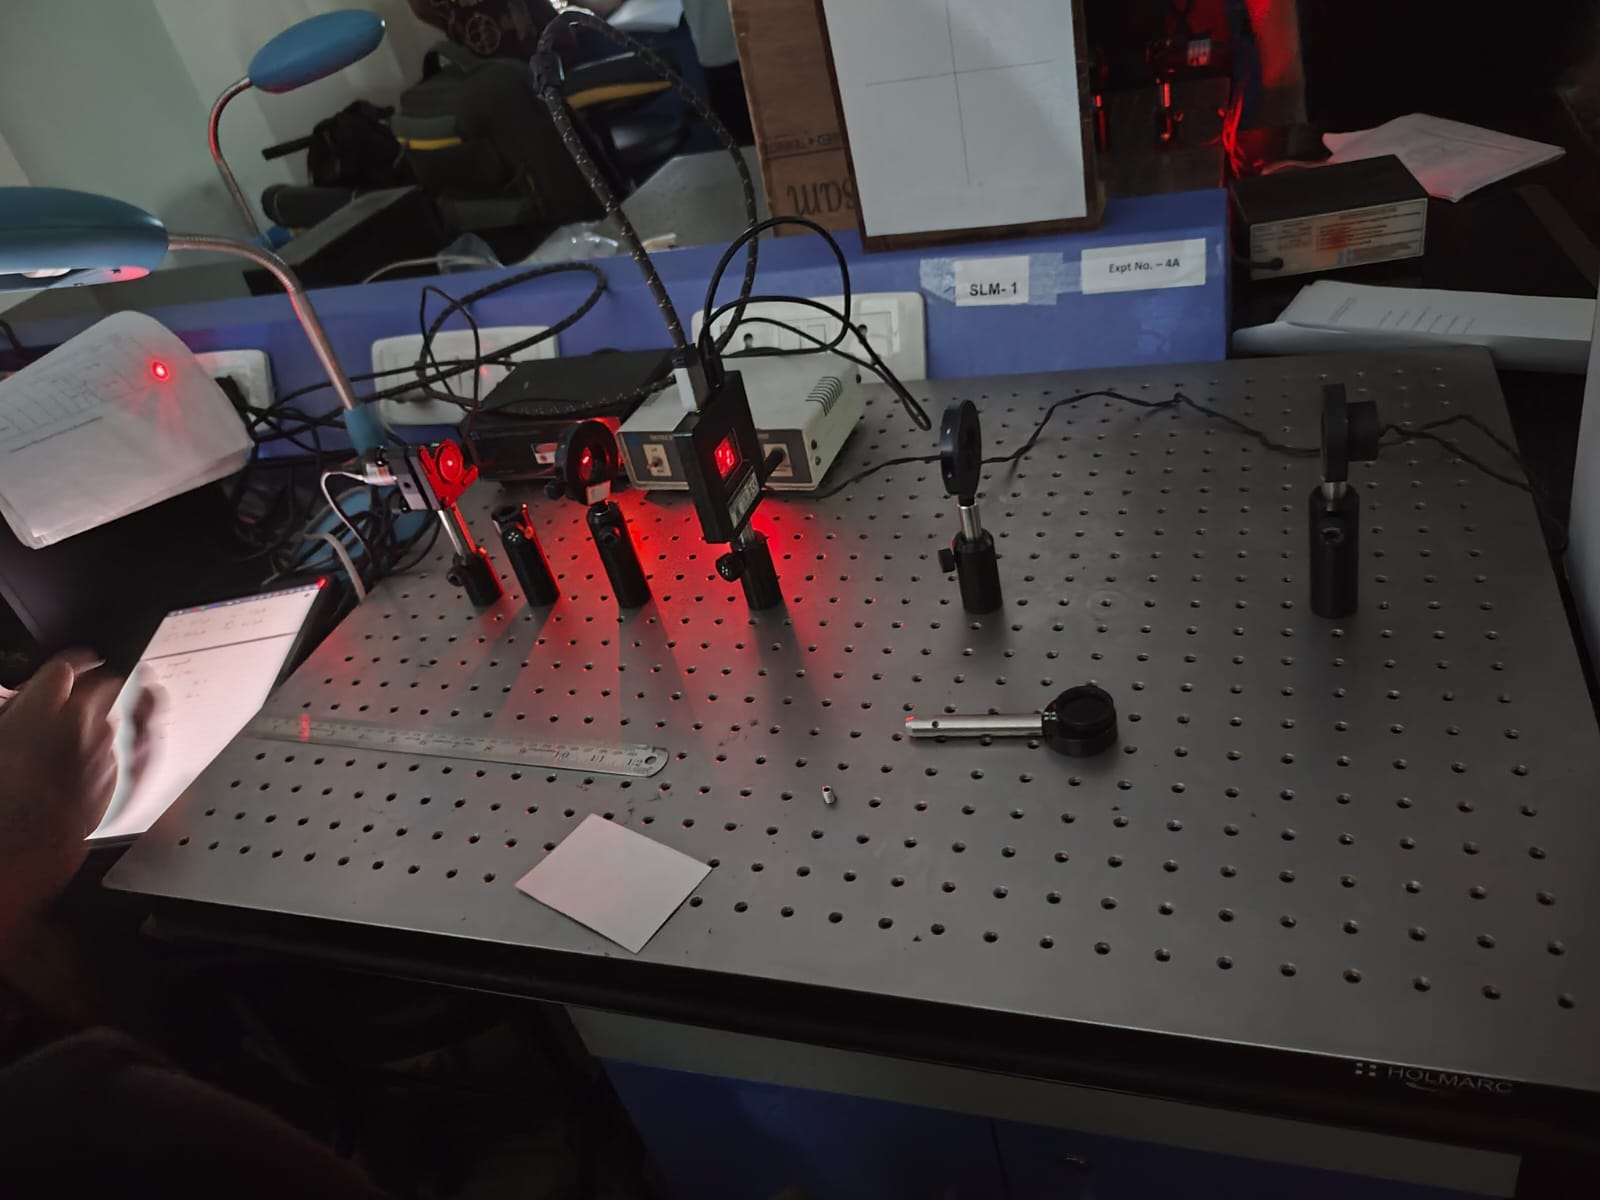
\includegraphics[width=0.5\textwidth]{setup.jpeg}
    \caption{Actual Experimental Setup}
\end{figure}


\section{Data}
\subsection{Calibration of Polarizer Axis}
The  reference angular positions corresponding to horizontal, vertical and the $\pm 45\degree$ polarization states by determination of \textit{Brewster's} angle.  Allowing the laser to fall on a air-glass interface, the angle of incidence was gradually varied while monitoring the reflected intensity. The angle corresponding to minimum reflected intensity was identified as \textit{Brewster's}
angle, when the reflected beam becomes purely \textit{s}-polarized, allowing identification of the horizontal axis of $P_1$. Then we placed the second polarizer in front of the first, to determine the vertical angular position of the second. The data is tabulated below.
\begin{table}[h!]
\centering
\begin{tabular}{c|c|c}
 & $P_1$ & $P_2$ \\
\hline
H & $284\degree$ 
  & $222\degree - 90\degree = 132\degree$ \\
\hline
V & $284 + 90\degree = 374\degree \equiv 14\degree$ 
  & $222\degree$ \\
\hline
P & $284+ 45\degree = 329\degree$ 
  & $132\degree + 45\degree = 177\degree$ \\
\hline
M & $284- 45\degree = 239\degree$ 
  & $132\degree - 45\degree = 87\degree$ \\
\hline
\end{tabular}
\caption{Polarization angle for $P_1$ and $P_2$}
\end{table}
\subsection{Measuring Polarization of SLM}
After calibration, we put the SLM in between the polarizers. Then we varied the grey scale and for each horizontal and vertical position of $P_1$, we aligned $P_2$ into the four polarization states and noted the intensity of the transmitted light. The data is tabulated below.
\begin{table}[H]
\centering
\begin{tabular}{c c c c c c}
\toprule
Grey Value & Input ($P_1$) & $I_H$ & $I_V$ & $I_P$ & $I_M$ \\
\midrule

0   & H & 3.9 & 5.1 & 3.6 & 1.6 \\
    & P & 16.8 & 40.8 & 2.4 & 51.4 \\

\midrule

64  & H & 0.8 & 2.4 & 2.5 & 1.3 \\
    & P & 16.6 & 19.1 & 17.0 & 32.2 \\

\midrule

128 & H & 0.4 & 4.0 & 2.7 & 1.5 \\
    & P & 12.3 & 39.2 & 2.6 & 50.0 \\

\midrule

255 & H & 0.5 & 3.7 & 2.7 & 1.4 \\
    & P & 15.3 & 39.6 & 15.3 & 50.5 \\

\bottomrule
\end{tabular}
\caption{Photodetector current for different grey values and polarization states.}
\end{table}
We calculate the Stokes vector from the data above, according to the given formulas.
\begin{table}[H]
\centering
\footnotesize
\renewcommand{\arraystretch}{0.8}
\begin{tabular}{c c c}
\hline
\textbf{Grayscale} & $\mathbf{P_1}$ & \textbf{Normalized Stokes Vector} $\vb{S}$\\
\hline
0   & Horizontal (H) & $\mqty[ 1 \\ -0.133 \\ 0.222 \\ - ]$ \\
0   & +45\degree State (P)      & $\mqty[ 1 \\ -0.416 \\ -0.850 \\ - ]$ \\

\hline

64  & Horizontal (H) & $\mqty[ 1 \\ -0.5 \\ 0.375 \\ - ]$ \\
64  & +45\degree State (P)      & $\mqty[ 1 \\ -0.07 \\ -0.426 \\ - ]$ \\

\hline

128 & Horizontal (H) & $\mqty[ 1 \\ -0.818 \\ 0.273 \\ - ]$ \\
128 & +45\degree State (P)      & $\mqty[ 1 \\ -0.522 \\ -0.920 \\ - ]$ \\

\hline

255 & Horizontal (H) & $\mqty[ 1 \\ -0.761 \\ 0.309 \\ - ]$ \\
255 & +45\degree State (P)      & $\mqty[ 1 \\ -0.443 \\ -0.641 \\ - ]$ \\

\hline
\end{tabular}
\caption{Normalized Stokes Vectors for Different Grayscale values}
\end{table}
\noindent
We then calculated $X$ and $Y$, from which we obtained $\delta$ and $\psi$, using the formulas mentioned before and then the extracted linear retardance and optical rotation were plotted as functions of greyscale values. 
\begin{figure}[H]
  \centering 
  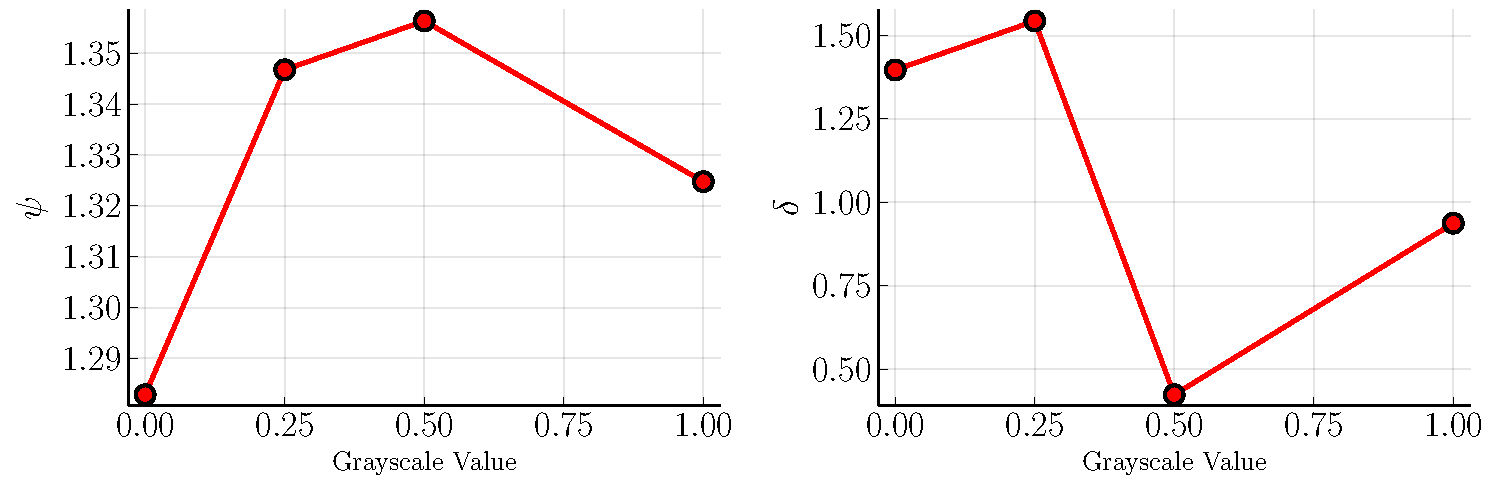
\includegraphics[width=0.9\textwidth]{SLM1.pdf}
\end{figure}


\section{Error Analysis}
\subsection{Random Error}
We analyze the errors introduced in the results. The Stokes' vectors were defined in Eq. \ref{stokes}. Using this, the uncertainty in the second component of the Stokes vector becomes, 
\begin{equation}
    \Delta [S]_2 = \abs{\frac{2I_V}{(I_H+I_V)^2}}\Delta I+\abs{\frac{2I_H}{(I_H+I_V)^2}}\Delta I = {\frac{2\Delta I}{(I_H+I_V)}}
\end{equation}
Simularly, for the third component we have the uncertainty 
\begin{equation}
    \Delta [S]_3 =  = {\frac{2\Delta I}{(I_H+I_V)}} +{\frac{2\abs{I_P-I_M}\Delta I}{(I_H+I_V)^2}} 
\end{equation}
Since $X$ and $Y$ are linearly related to these components, we get the uncertainty in $X$ and $Y$ just by adding these uncertainities. From that, we obtain the uncertainty in $\psi$ and $\delta$. 
\begin{align*}
    \psi = \frac{1}{2}\tan^{-1}\qty(\frac{Y}{X}) \implies \pdv{\psi}{X} = -\frac{Y}{2(X^2+Y^2)}\quad \pdv{\psi}{Y} = \frac{X}{2(X^2+Y^2)}\implies \Delta \psi = -\frac{|Y|\Delta X}{2(X^2+Y^2)} +  \frac{|X|\Delta Y}{2(X^2+Y^2)}
\end{align*}
Similarly, if we do this for the linear retardance we get, 
\begin{align*}
    \delta =\cos^{-1}\qty(\sqrt{X^2+Y^2}-1)\implies \Delta \delta  = \frac{|X|\Delta X + |Y|\Delta Y}{\sqrt{X^2+Y^2}\sqrt{1 - (\sqrt{X^2+Y^2}-1)^2}}
\end{align*}
The least count of the photodetector was $0.1\ \mu A$ which implies $\Delta I =0.1\ \mu A$. Using these formula above, we get the maximum possible errors for each greyscale value as, 
\begin{table}[H]
\centering
\begin{tabular}{c|c|c}
 Grayscale & $\Delta\psi$  (rad.) & $\Delta \delta$ (rad.) \\
\hline
0 & $0.016$ 
  & $0.036$ \\
\hline
64 & $0.054$ 
  & $0.098$ \\
\hline
128 & $0.02$ 
  & $0.163$ \\
\hline
255 & $0.026$ 
  & $0.09$ \\
\end{tabular}
\end{table}
\subsection{Sources of Error}
\begin{itemize}
  \item The laser was not stable at all times which could have led to fluctuations in the measured internsity.
  \item The polarizers were not perfect, hence there was always some residual component from the unintended polarization states which could have introduced errors.
  \item The SLM crystals might have some spatial non-uniformity which could have caused error in measurement. 
  \item The variation in external temperature could have affected the SLM crystals, leading to some error. 
\end{itemize}

\section{Discussion and Conclusion}
The variation of linear retardance ($\delta$) and optical rotation ($\psi$) with grayscale demonstrates that the SLM effectively modulates the polarization state of light. The observed dependence is clearly non-linear, which is expected due to the nonlinear electro-optic response of liquid crystal molecules to the applied voltage.\\[0.2cm]
The retardance shows a smooth variation with grayscale, indicating controlled phase modulation. In contrast, the optical rotation exhibits a non-monotonic behavior, reflecting the complex interplay between birefringence and molecular reorientation within the SLM.\\[0.2cm]
Uncertainty analysis shows that the error in $\delta$ is significantly larger than that in $\psi$. This arises from the higher sensitivity of the inverse cosine function used in calculating retardance, making it more susceptible to small fluctuations in measured intensities.\\[0.2cm]
Deviations from ideal behavior can be attributed to experimental limitations such as polarizer misalignment, finite extinction ratio, laser intensity fluctuations, and non-uniformity of SLM pixels. Despite these factors, the overall trends remain consistent and physically reasonable.\\[0.2cm]
In this experiment, we studied the polarization properties of a SLM using Stokes polarimetry. The linear retardance ($\delta$) and optical rotation ($\psi$) were extracted for different grayscale values from measured intensity data.\\[0.2cm]
The measured values indicate that the SLM introduces significant phase retardation and polarization rotation, both of which vary with the applied grayscale. The estimated uncertainties were $\Delta \psi \approx 0.016$ to $\Delta \psi \approx 0.054$ rad and $\Delta \delta \approx 0.036$ to $\delta \approx 0.163$ rad within the values of the grayscale measured. The larger uncertainty in $\delta$ is consistent with the higher sensitivity of the inverse cosine function used in its calculation.\\[0.2cm]
Overall, the results confirm that the SLM acts as a voltage-controlled birefringent element capable of modulating both phase and polarization of light. The observed trends and magnitudes are consistent with the expected nonlinear electro-optic response of liquid crystal systems.\\[0.2cm]
\end{document}


